\chapter{Risultati Sperimentali}
In questo capitolo vengono discussi i risultati degli esperimenti effettuati sul sistema.\\*
Gli esperimenti sono divisi principalmente in due categorie:
\begin{itemize}
	\item Esperimenti \emph{offline}:\\*
	I dati di accelerazione, velocit\`a angolare, velocit\`a lineare e posizione vengono generati attraverso RTT e passati a un'istanza locale di \texttt{FusionLib}.\\*
	I risultati forniti da SFA vengono mostrati su RTT in forma grafica.\\* Questi esperimenti sono essenzialmente \emph{Integration Test} volti a validare l'implementazione di SFA.
	\item Esperimenti \emph{online}:\\*
	Il software che genera i dati si comporta come un'astrazione di \texttt{interface-modules}, e le misurazioni prodotte vengono inviate in accordo a \texttt{INPUT\_PROTOCOL} a una scheda \texttt{NVidia TX-Jetson} su cui \`e replicato l'ambiente HW e SW bordo treno. Tali dati sono inviati alla scheda attraverso un'interfaccia \texttt{ethernet}, utilizzata in luogo dell'interfaccia \texttt{loopback} prevista dal sistema reale.\\*La scheda invia i dati in uscita da SFA ,attraverso la medesima interfaccia \texttt{ethernet}, al mittente dei dati in entrata in accordo a \texttt{OUTPUT\_PROTOCOL}.\\*In questo caso, l'interfaccia \texttt{ethernet} sostituisce l'utilizzo del modem \texttt{LTE}.\\*
	Questi esperimenti sono essenzialmente \emph{End to End Test} e hanno lo scopo di validare i protocolli di comunicazione.
\end{itemize}
La linea ferrotramviaria scelta come ambiente di prova \`e la linea \texttt{T1} della Tramvia di Firenze, che collega la stazione di \emph{Villa Costanza}, sita nel comune di Scandicci, all'ospedale di \emph{Careggi}, sito quest'ultimo nel comune di Firenze. La linea \`e mostrata in figura \ref{fig:t1}.\\*
\begin{figure}[h]
	\centering
	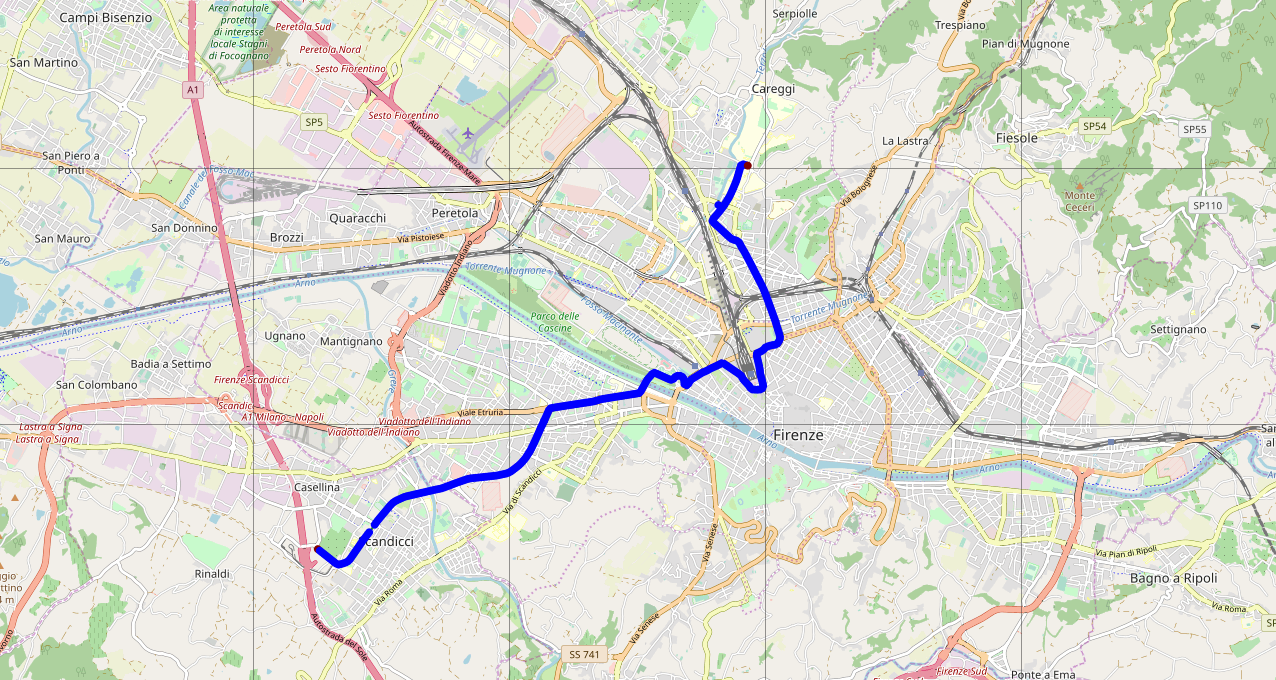
\includegraphics[width=\linewidth]{img/t1}
	\caption{Tramvia di Firenze - Linea \texttt{T1}}
	\label{fig:t1}
\end{figure}
\section{Software impiegati}
In questa sezione vengono descritti i SW utilizzati negli scenari sopra descritti.
\subsection{FusionLib}
Come accennato nel Capitolo 3, \texttt{FusionLib} \`e una \emph{libreria software} che implementa SFA. Tale libreria viene compilata sia su \texttt{Windows 10}, su cui esegue RTT, che su \texttt{Ubuntu 16.04 LTS}, su cui esegue \texttt{listener}. \texttt{FusionLib} \`e pertanto una libreria inclusa da \texttt{listener} e RTT.\\*
Per determinare la posizione del treno lungo la traccia \texttt{FusionLib} utilizza le informazioni ricevute dal chiamante combinate con le informazioni della traccia su cui si assume il treno si stia muovendo. Tali informazioni sono salvate in un \emph{database} cui la libreria accede per mantenere la consistenza fra stima della distanza percorsa, posizione geografica assoluta e progressiva chilometrica. Lo schema logico \`e riportato in figura \ref{fig:fulib}.
\begin{figure}[h]
	\centering
	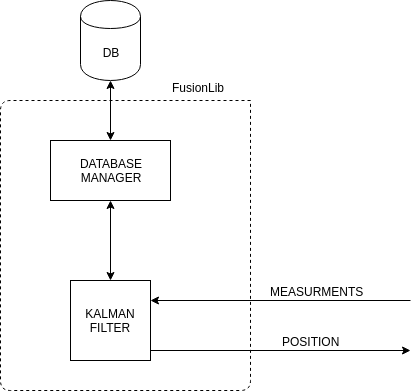
\includegraphics[width=\linewidth]{img/fulib}
	\caption{Architettura logica di \texttt{FusionLib}}
	\label{fig:fulib}
\end{figure}
\subsection{RTT}
RTT ha una doppia funzionalit\`a, infatti permette sia di interfacciarsi a un'istanza esterna di \texttt{FusionLib} per tracciare il treno su una mappa, sia di generare i dati dei sensori, salvarli nel database, e recuperarli per testare l'algoritmo in un successivo momento.
